\documentclass{beamer}[10]
\usepackage{pgf}
\usepackage[danish]{babel}
\usepackage[utf8]{inputenc}
\usepackage{beamerthemesplit}
\usepackage{graphics,epsfig, subfigure}
\usepackage{url}
\usepackage{srcltx}
\usepackage{hyperref}
\usepackage{graphicx}
\usepackage{multirow}
\usepackage{xcolor}

\graphicspath{ {images/} }

\definecolor{kugreen}{RGB}{0,53,24}
\definecolor{kugreenlys}{RGB}{132,158,139}
\definecolor{kugreenlyslys}{RGB}{173,190,177}
\definecolor{kugreenlyslyslys}{RGB}{214,223,216}
\setbeamercovered{transparent}
\mode<presentation>
\usetheme{PaloAlto}
\setbeamertemplate{footline}[page number]
\setbeamerfont{footline}{size=\tiny}
\setbeamercolor{footline}{fg=white}
\setbeamertemplate{navigation symbols}{}


  %\useoutertheme{default}
  \usecolortheme[named=kugreenlys]{structure}
  \useinnertheme{circles}
  \usefonttheme[onlymath]{serif}
  \setbeamercovered{transparent}
  \setbeamertemplate{blocks}[rounded][shadow=true]

\logo{
\includegraphics[width=1.5cm]{Uoseal.png}}
%\useoutertheme{infolines} 
\title{}
\subtitle{\huge{Using Statistical Distributions to Generate Random Test Data}}
\author{Jamie L. Zimmerman}
\institute{Robert D. Clark Honors College \\ Department of Computer and Information Science \\ University of Oregon}
\date{25 May 2018}

\AtBeginSection[]
{
  \begin{frame}
    \frametitle{Overview}
    \tableofcontents[currentsection]
  \end{frame}
}


\begin{document}
\frame{\titlepage \vspace{-0.5cm}
}

%introduction

Software testing is a crucial part of systems that run our lives. Industries that rely on predicting consumer habit trends or dispatching taxi cars are terribly effected when their software fails to provide accurate results. The gravity of this trust is even greater in safety-critical programs controlling gas-leak shut off valves or anesthetic delivery machines. Consequently, before these pieces of software are deployed, they must be checked and tested rigorously. The breadth and completeness of testing is directly proportional to how much damage could occur if the software malfunctioned. The software must eventually reach production (used in the hands of the customer or in industrial practice ``for real'') which means that it has to leave the testing stage eventually. When that time comes, testers must be assured that the software behaves properly. This only sometimes happens. A 2017 report found that 43\% of software engineers did not have enough time to test their code before its release date~\cite{Kassab-deFranco-Laplante}. Therefore, the tradeoff of cost and convenience is an important consideration in determining the rigor of testing. When the release date occurs, testers either have to ship their product without confidence it works or else invest extra time and energy into seeing it does work. Cost is never low, and convenience is never high, so software testing remains a lengthy and sometimes ad hoc practice in many industrial applications. Numerous papers agree that  testing is a tremendously arduous part of software development~\cite{Murphy:2007:PRT:1292414.1292425,Haller:2010:TDC:1838126.1838132,Muslu:2015:PDE:2771783.2771792,Tiwari:2013:RRT:2439976.2439982,Gupta:2011:MBA:2002931.2002932,Zeller:2017:STS:3105427.3105438,Garousi:2017:IWA:3084226.3084264,Kassab-deFranco-Laplante,Langdon:2017:IAT:3105427.3105429,Goffi:2016:AGO:2931037.2931061}. In fact, Misailovic et. al report that 50\% of the software development process is software testing. This is not surprising since testing the quality of software is inherently an impossible solution.

Firstly, testing the software means knowing what the software \textit{should} do and what output it \textit{should} generate. A key component of getting correct results is knowledge of what correctness looks like. Developers and testers must be careful not to confuse code that compiles and runs without errors with code that renders accurate results. To find accurate results, testers need an oracle, which is a way of determining how close the actual result of a program is to the expected result. Figure \ref{fig:workflow} illustrates the divergence. Unsurprisingly, obtaining and checking this oracle is difficult. Given a particular input to a program, a tester must know what the expected result even is. 
\begin{wrapfigure}{l}{0.65\textwidth}
\centering
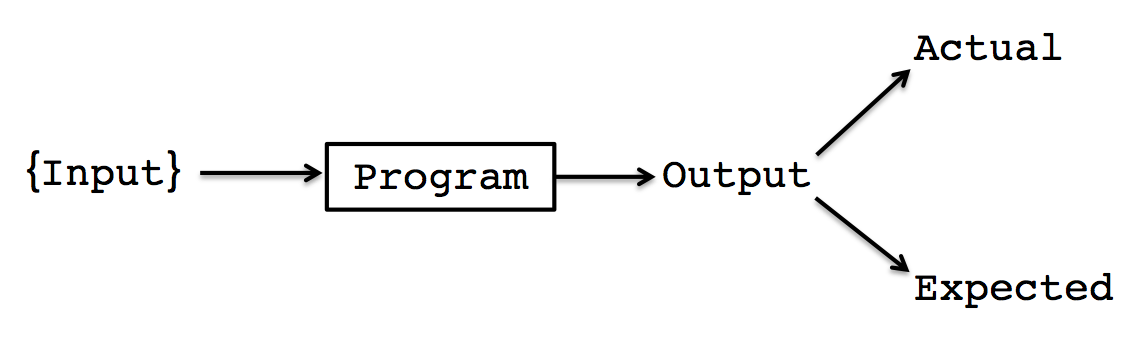
\includegraphics[width=90mm,scale=0.5]{diagram.png}
\caption{Basic Workflow of a software program}
\label{fig:workflow}
\end{wrapfigure}
Then, she must know how to read or understand the actual result and be able to compare it to the expected.\footnote{Consequently, many companies often build the role of tester into the role of developer, since the developer has the most intimate knowledge of the design and implementation of the software, and therefore has a better sense of what the output of the program exhibits. Even then, it may be impossible to describe the ideal expected output of the program.} In immensely complex scientific software or finanical programs swathed in accounting terms, the output of the program might be an unknown language to the tester. Even if the tester is a domain scientist, the output may be too complicated to read quickly and identify the trends that indicate she received a postive test result.

Another major challenge in software testing is the need to know all the possible situations one may want to test for. In an automobile simulator, for example, a tester does not want to just test for braking and accelerating, she wants to test turn-signaling, beeping, and brake-lighting, and also combinations of those tests to make sure that the beeping sensor does not accidentally disable the brake pedal capability. Knowing and describing every single situation may be unknown to the tester; they may not even think that that is a situation they have to test for. But these situations must be tested. What is known as the ``happy path'', the operational choice that most frequently represents the typical testing scenario, is certainly necessary for testing the program’s reliability, but it does not find the bugs. Outlier situations find the bugs. Lindvall et. al summarize the need for edge cases in their research in testing autonomous drones: ``Just because the drone behaves in a safe manner for a set of test scenarios does not mean that it will always behave in a safe manner for other scenarios''~\cite{Lindvall:2017:MMT:3103620.3103632}. Identifying all these possible outlier situations is \textbf{Problem One}.

With human's prolific ability to create and store data quantifying the world around them, it is hard to imagine that a tester could not find data that they could use. Gotterbarn agrees that ``Insufficient data is not a problem''~\cite{Gotterbarn:2016:CFC:2874239.2874248}. For example, consider an ocean temperature monitoring software that has predictive power in future local hot spots or cold zones. Ocean temperature data points do exist, and the missing points can likely be interpolated quite easily. But this is a sample size of one. To be sure the temperature projection software is robust, the tester would want to study a variety of circumstances and possibilities – situations that do not even exist. They might perhaps want to study temperature diffusion trends as a result of a hypothetical significant event 30 years from now. Data for that particular test case has to be created.

This is \textbf{Problem Two} -- writing the actual test data itself. A symbolic description of the test must be turned into an actual concrete input to the software. A test vector checking that beeping does not disable braking must be turned into ``beeping=5s\&\&braking=true'' or whatever discrete format the SUT requires. This is not a step that should be done manually. For example, VisIt, a graphical visualization tool, is capable of handling several gigabyte files~\cite{VisIt}. No tester wants to or even could write three gigabytes of data points modeling a real-world situation by hand just to satisfy one test case. Nearly every software testing paper agrees that writing data by hand seriously hinders the testing process~\cite{Misailovic:2007:PTG:1287624.1287645,Murphy:2007:PRT:1292414.1292425,Palka:2011:TOC:1982595.1982615,Patrick:2016:ATI:2970276.2970333}.

It is significantly easier to describe the trend of a certain test than it is to create the hundreds (if not more) data points that fit that description. Therefore, the goal of this project is to bridge that gap. It aims to aid the tester in designing and creating test suites so as to provide automation in the testing process. Automation, simplicity, and ease of use are key tenets of this project. Making a tester's job easier is much more likely to help them do it well, and making this tool accessible and easy to use is a low-cost, high-convenience solution that not only codifies a standardized testing procedure but shortens the duration of the testing phase and ensures resilient software before its deployment date. 

%proprosed argument
I believe that I have designed an approach to these problems and have architected a simplistic solution that automates the steps described in the introduction. I hypothesize that Problem One is solved by the advent of combinatorial testing, which identifies most, if not all, of the test cases necessary for confidence in working software. My tool, Parmgen, has solved the second problem, translating the English description of a test case into a concrete format that can be used as input into the program. I ask the user for smaller, more simplistic descriptions of their input data, which requires less work than writing every data point by hand. Then I can use Python's random statistical distributions to generate those points and write them to a convenient location for the tester’s use. This tool is written in the Python language, which is useful for prototyping the MVP (Minimum Viable Product) of this tool. I call this entire pipeline GenSequence.

% Design Decisions
\section{Architecture}

\frame{
\frametitle{Pairwise Testing}
\begin{figure}
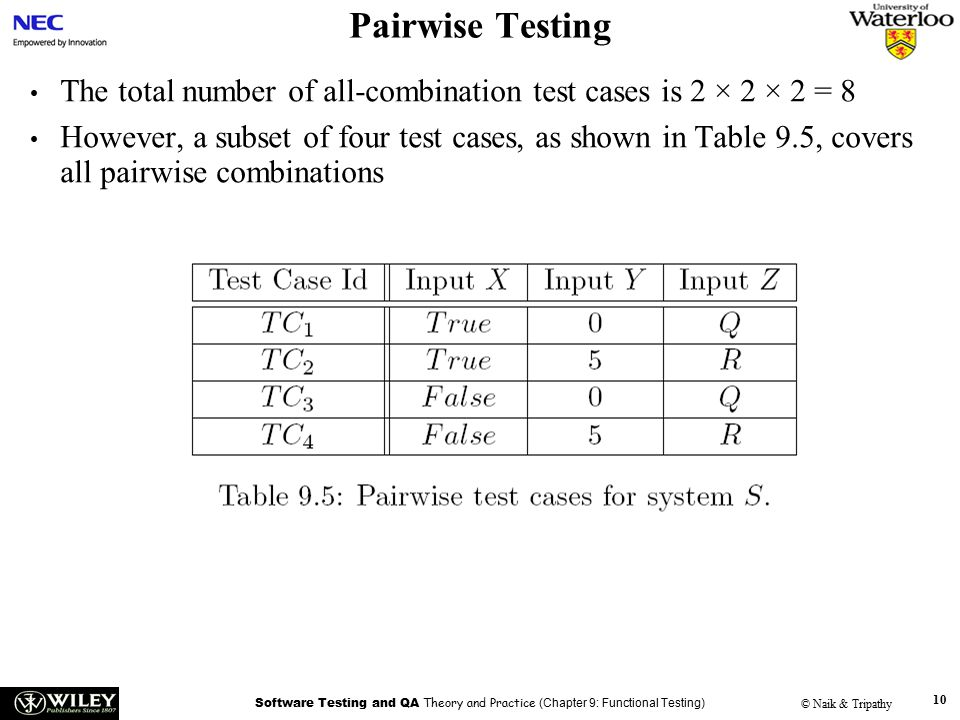
\includegraphics[scale=0.4]{pairwise.jpg}
\end{figure}
}

\frame{
\frametitle{ParmGen}
\begin{table}
\begin{tabular}{l | c | c}
\emph{Item Purchased} & \emph{Price} & \emph{Delivery Method} \\
\hline \hline
{\color{red}Large Item} & {\color{red}Expensive} & Lightspeed \\ 
Small Item & Mid-price & SnailMail \\
ExtraSmall Item & Cheap & {\color{red}Ultrafast} \\
\end{tabular}
\caption{Possibilities}
\end{table}

\begin{table}
\begin{tabular}{l | c | c}
\emph{Item Purchased} & \emph{Price} & \emph{Delivery Method} \\
\hline \hline
Boat & \$10,000.00 & Space Rocket \\
\end{tabular}
\caption{Concrete Test Vector}
\end{table}
}

\frame{
\frametitle{ParmGen Space}
\begin{columns}
    \begin{column}{0.48\textwidth}
        \begin{table}
        \begin{tabular}{l | c}
        \emph{Cats} & \emph{Dogs} \\
        \hline \hline
        10 & 1 \\
        \end{tabular}
        \caption{Unit Parameter}
        \end{table}
    \end{column}
    \begin{column}{0.48\textwidth}
        \begin{table}
        \begin{tabular}{l | c}
        \emph{Cats} &  \emph{Dogs}\\
        \hline \hline
        10 & 1 \\ 
        1 & 1 \\ 
        10 & 10 \\ 
        10 & 100 \\ 
        10 & 1 \\ 
        1 & 10 \\ 
        10 & 10 \\ 
        10 & 1 \\ 
        1 & 1 \\
        10 & 100 \\
        100 & 1 \\
        1 & 10 \\

        \end{tabular}
        \caption{System Parameter}
        \end{table}
    \end{column}
\end{columns}
}

\frame{
\frametitle{ParmGen Space}
Cats is \emph{not} just 100. \\
\vspace{1cm}
Cats is [10, 1, 10, 10, 10, 1, 10, 10, 1, 10, 100, 1, ...] \\
\pause
\vspace{1cm}
Cats is [1, 2, 2, 3, 3, 3, 4, 3, 2, 1, 1]
}


\frame{
\frametitle{100 points -- average $=$ 15, std. deviation $=$ 5}
\begin{figure}
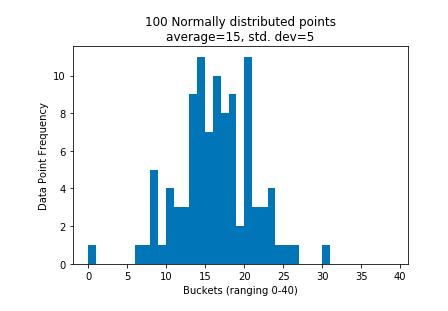
\includegraphics[scale=0.6]{law1.png}
\end{figure}
}

\frame{
\frametitle{Law of Large Numbers}
\begin{itemize}
\item Bernoulli's Principle
\item Selection Scheme
\end{itemize}
}

\frame{
\frametitle{10,000 points -- average $=$ 15, std. deviation $=$ 5}
\begin{figure}
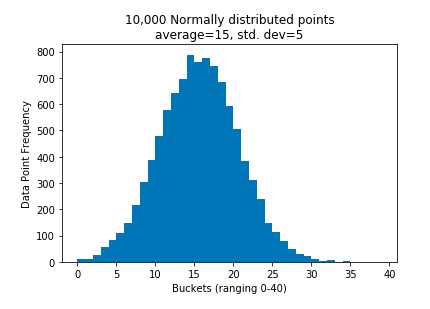
\includegraphics[scale=0.6]{law2.png}
\end{figure}
}

\frame{
\frametitle{300 points -- average $=$ 15, std. deviation $=$ 5}
\begin{figure}
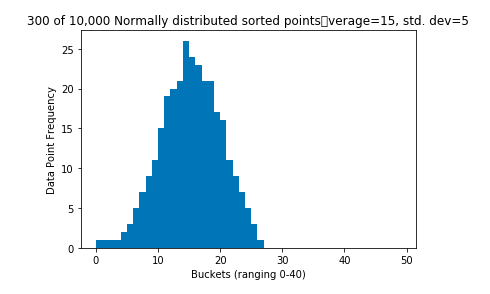
\includegraphics[scale=0.6]{law3.png}
\end{figure}
}

\frame{
\frametitle{A Variety of Statistical Distributions}
\begin{figure}
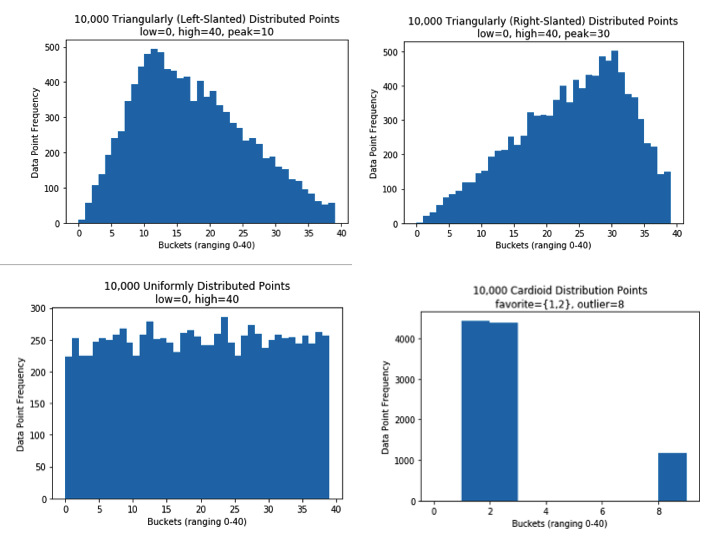
\includegraphics[scale=0.4]{distributions.png}
\end{figure}
}

\frame{
\frametitle{Cardioids}
$$r = \alpha \pm \alpha cos \theta$$
\begin{figure}
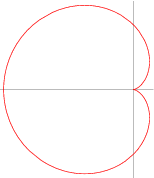
\includegraphics[scale=0.9]{cardioid.png}
\end{figure}
}

\frame{
\frametitle{Preprocessor}
\begin{figure}
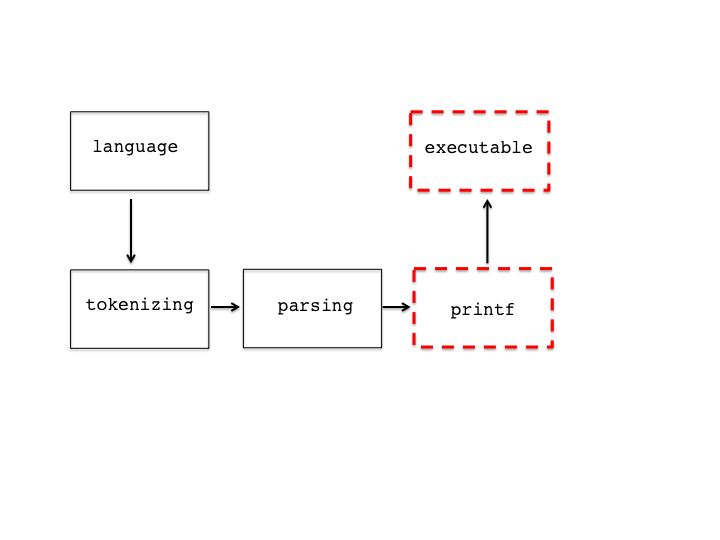
\includegraphics[scale=0.45]{preprocess.png}
\end{figure}
}

\frame{
\frametitle{GenSequence}
\begin{figure}
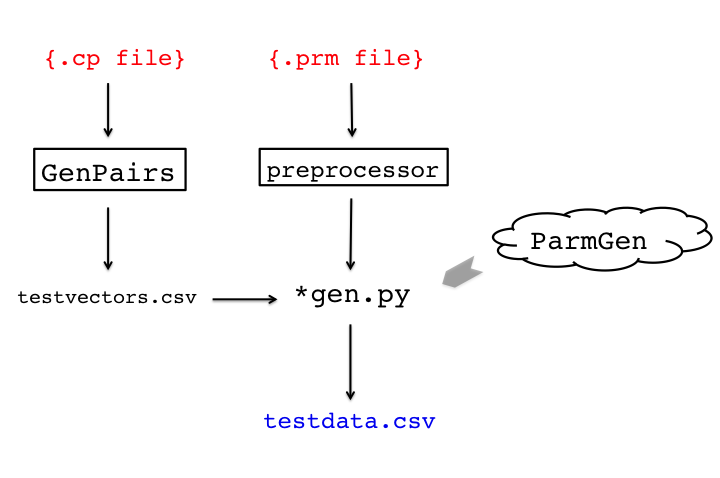
\includegraphics[scale=0.4]{workflow.png}
\end{figure}
}

\frame{
\frametitle{}
\begin{figure}
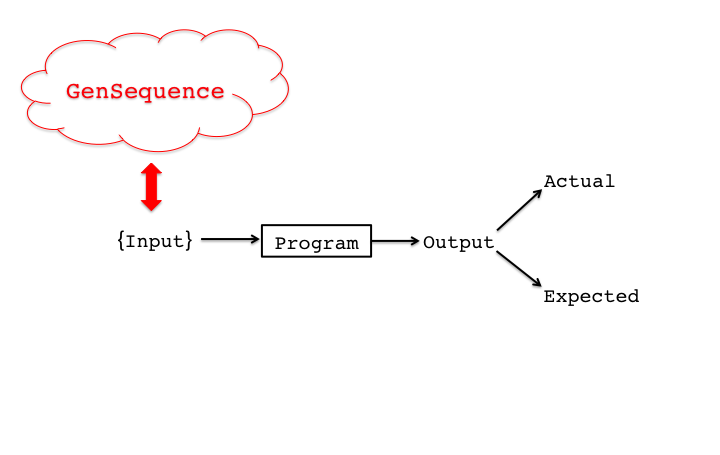
\includegraphics[scale=0.4]{diagram2.png}
\end{figure}
}

%results
\section{Celestial Body Simulation}
Initial use of GenSequence on the planetary orbits program proved some promise in the capability of this tool. I used the tool to generate 30 test cases. Test case 13 was programmatically named:
\vspace{1cm}

\noindent\fbox{
    \parbox{\textwidth}{
        {\fontfamily{pcr}\selectfont
        13-70-mass|right_slanted-position|right_slanted-velocity|uniform-diameter|left_slanted.csv
        }
    }
}

\vspace{1cm}
13 describes the test case number, 70 describes the number of rows in the test case. In this simulation, each row represents an instance of a planetary body.

Planetary masses were generated with a right slanted distribution. Position, the location of each body, was generated with a right-slanted triangular probability. The velocities of the bodies were generated uniformly. The diameters, the visible size in the program's GUI, were generated by a left-slanted distribution. The starting point of this program's test data showed this visualization:

\begin{figure}[h!]
\centering
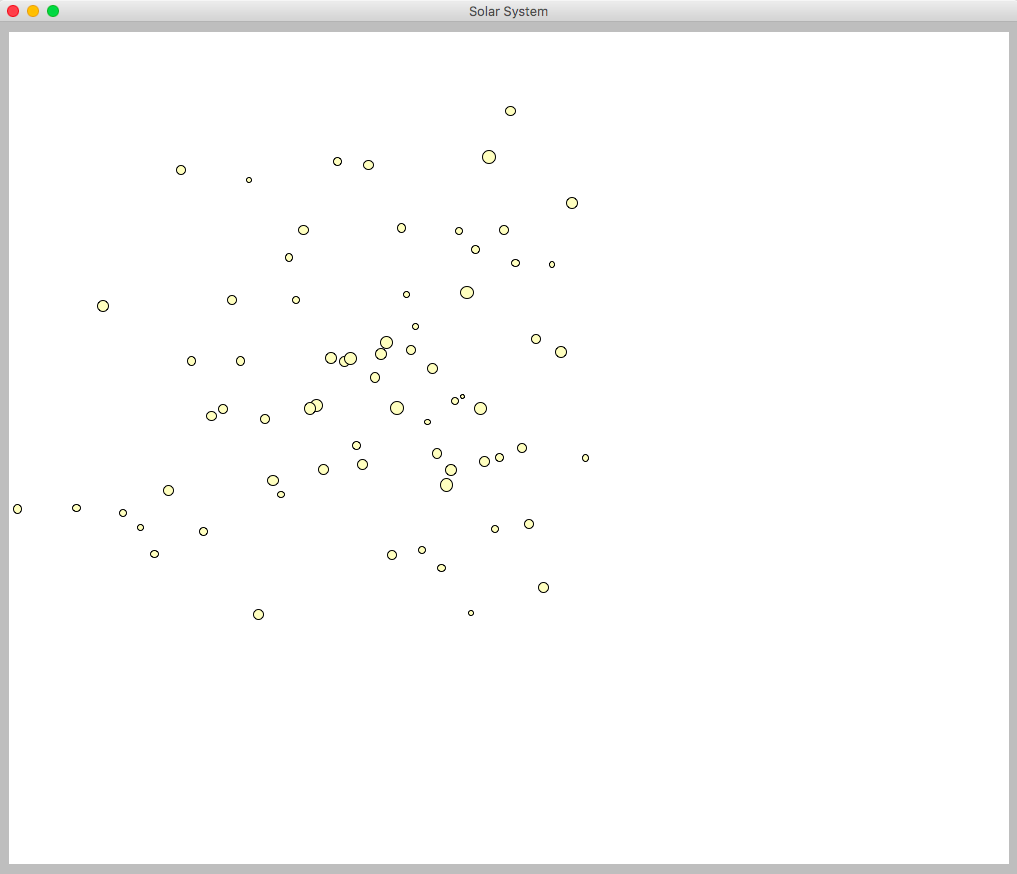
\includegraphics[scale=0.4]{start-ex.png}
\caption{Starting Locations of 70 celestial bodies}
\label{fig:startbody}
\end{figure}

Figure \ref{fig:startbody} accurately reflects the visible parameters – position and diameter. The positions were generated by a right slant, and ostensibly so, the bodies are mostly located in one region. The diameters were generated by a left-slanted distribution, clearly slanted towards a smaller diameter, with most samples appearing small or medium size, but a notable number appearing fairly large.

The program by nature tracks and draws the motion of each planetary body through time, giving a useful summary of the program’s execution by the end of the simulation (665 time steps). Running test case 13 garnered Figure \ref{fig:endbody}.

\begin{figure}[h!]
\centering
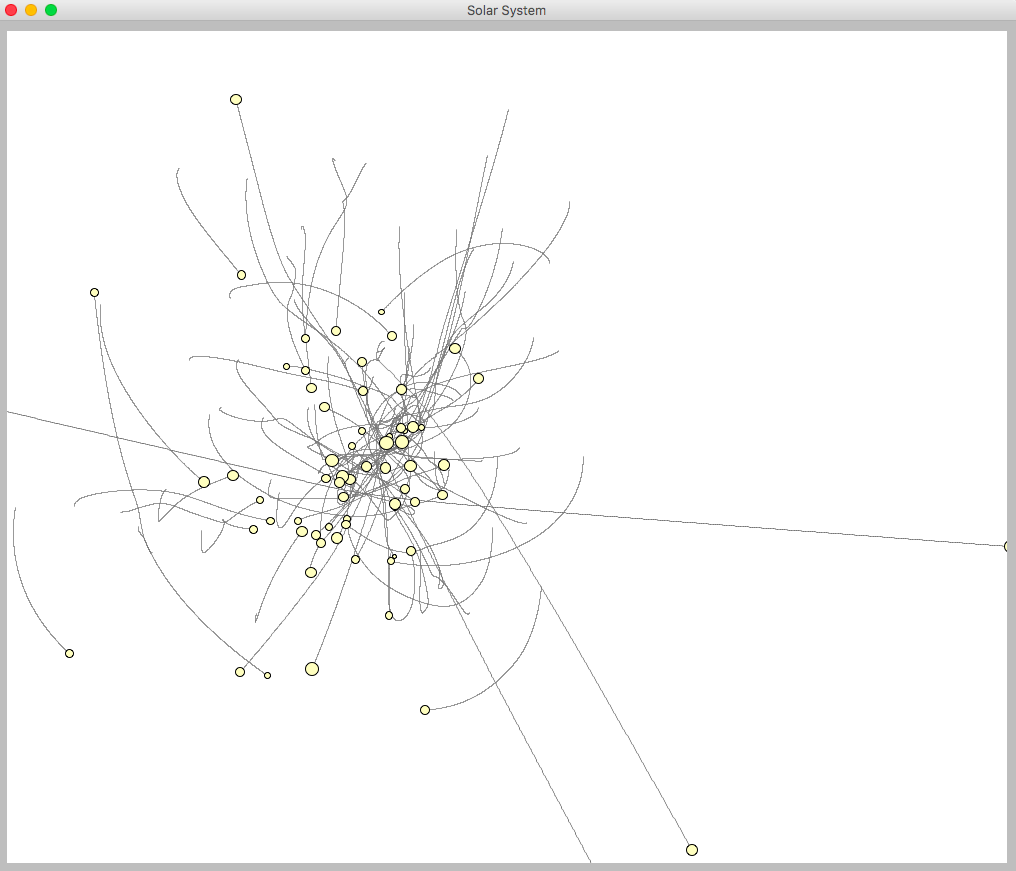
\includegraphics[scale=0.4]{final-ex.png}
\caption{Ending Locations of 70 celestial bodies after 665 time steps}
\label{fig:endbody}
\end{figure}

Spending a minute closely observing these paths registers some important observations about the natural behavior of gravity acting on planetary bodies. Some disobeyed their trajectory and were redirected by the large mass in the center. The initial velocities manifested themselves as well. The paths are of all different lengths, which makes sense since they were generated by a uniform distribution.

\section{Earthquake Analysis and Visualization Program}
The earthquake analysis program performs basic statistical analysis of magnitudes, locations, and depths on a map, and also plots quake events on a map. Bigger dots represent a greater data point value (This is important to note because dots representing magnitudes describe their intensity not their destruction coverage). One test case had a file name (test vector) of:
\vspace{1cm}

\noindent\fbox{%
    \parbox{\textwidth}{%
        {\fontfamily{pcr}\selectfont
        6-70-magnitudes|cardioid-latitudes|left_slanted-longitudes|right_slanted-depths|cardioid.csv
        }
    }%
}

\vspace{1cm}
Observing the cardioid relationship between latitudes and longitudes is confirmation of GenSequence working. GenSequence was programmed with the following information:
\vspace{1cm}

\begin{lstlisting}
#magnitudes ranges
Micro = Range(0.0, 2.0, exclusive_upper=True)
Feelable = Range(4.5, 7.9, exclusive_lower=True)
Great = Range(8.0, 9.5, exclusive_lower=True, exclusive_upper=True)
#depths ranges
Shallow = Range(0.0, 5.0, exclusive_lower=True, exclusive_upper=True)
Mid = Range(5.0, 15.0)
Deep = Range(15.0, 30.0, exclusive_lower=True)
...
# specify the relationship between magnitudes and depths
MagsDepths = Cardioid(Mags, Depths)
MagsDepths.setFavorites([(Micro,Shallow), (Great,Deep), (Feelable,Mid)])
MagsDepths.setNonFavorites([(Micro,Deep), (Great,Shallow), (Feelable,Deep), (Feelable,Shallow)])
\end{lstlisting}

\vspace{1cm}
This is the literal implementation of the tool describing the most frequently occurring data pairs in this test case. Low intensity magnitudes should be near Earth’s surface and very intense magnitudes should occur deep below the earth’s surface. Moreover, it is not very frequent that low-intensity earthquakes occur very deeply, and high-intensity earthquakes occur very near surface. \footnote{This assumption may be entirely false about the nature of earthquakes. This trend is one I invented to add functionality to GenSequence, one that could easily be reversed by any seismologist user of the program.}

The plots of magnitudes and depths (Figure \ref{fig:magsdepths}) show this constraint propagating:
\begin{figure}[h!]
  \centering
  \begin{subfigure}[b]{0.6\linewidth}
    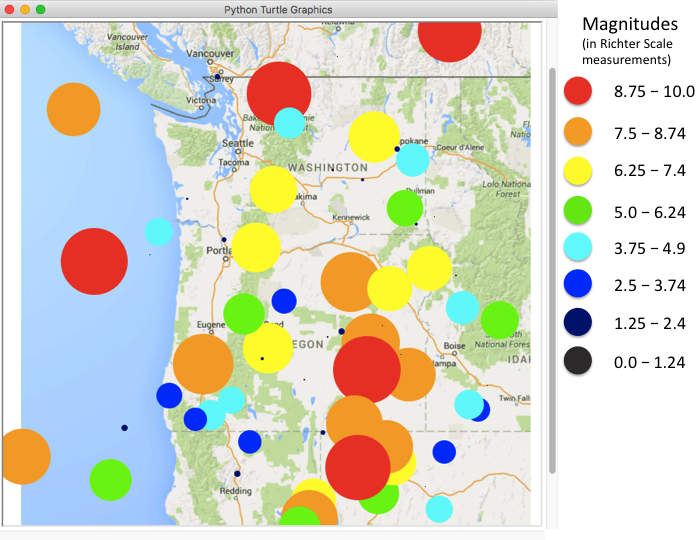
\includegraphics[width=\linewidth]{mags.png}
    \caption{Magnitudes}
  \end{subfigure}
  \begin{subfigure}[b]{0.6\linewidth}
    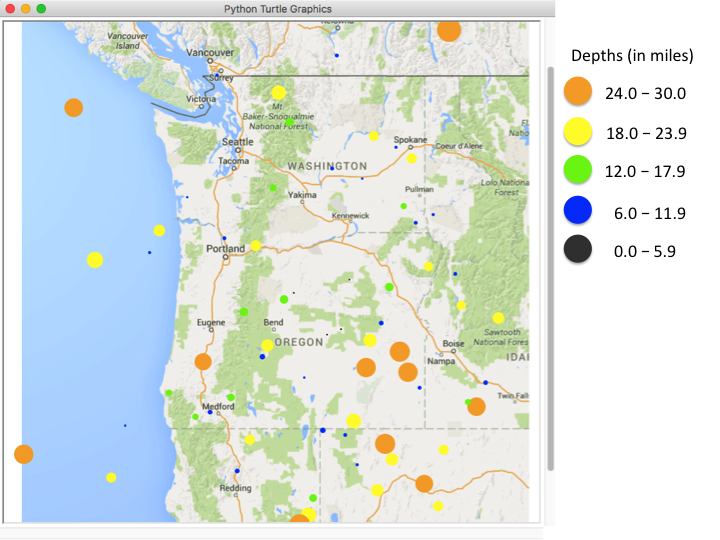
\includegraphics[width=\linewidth]{depths.png}
    \caption{Depths}
  \end{subfigure}
  \caption{Plotting Magnitudes and Depths from the same test case}
  \label{fig:magsdepths}
\end{figure}

The correlation is rather difficult to piece but does reflect exactly what is expected. The large red dot due west of Portland has a matching yellow depth dot. The small blue event due west of the Oregon-California border has a matching blue dot in the same place. One outlier is a sizable orange earthquake covering the Umatilla forest that has a very tiny blue depth dot.

Considering latitude-longitude oriented north-up, west-left, east-right, south-down, and given the left-slanted-ness of the latitudes and right-slanted-ness of longitudes, this test case should mark the locations of the earthquakes mostly drifting towards the lower-right corner. This is in fact what the program generates (Figure \ref{fig:clusters}).

\begin{figure}
\centering
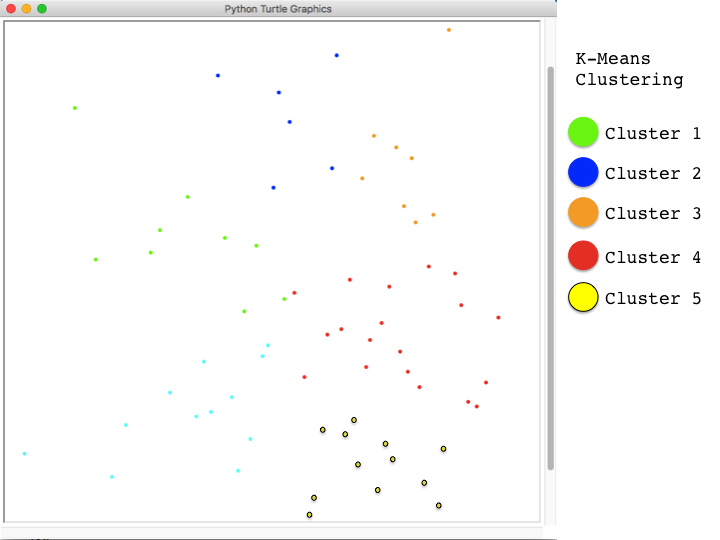
\includegraphics[scale=0.5]{clusters-nobg.png}
\caption{K-Means Clustering of Earthquake events from case 13}
\label{fig:clusters}
\end{figure}

%conclusion

I believe that GenSequence's best application is for testing database-driven applications. These applications literally control the world. Consider financial applications alone: the record of every transaction, every payment, every credit report, and every bill can dictate a person’s entire life. The infrastructure surrounding that data must not expunge or fabricate any of it, and must maintain its integrity. Software that accesses, controls, and manipulates this huge amount of data carries substantial responsibility. Moreover, software that can read, interpret, and identify trends in a huge wealth of global data has amazing power in informing us of what happens in the world and how we can make better decisions. It is therefore of utmost importance to design that software well enough to trust its results.

GenSequence has addressed those demands. It functions simply but provides automation during the testing stage and generates reliable data that is what is says it is. If the context of the program warrants consideration of statistically unlikely but possible scenarios, GenSequence can make that happen. It primarily states its power by its ease of use and nearly end-to-end automation. Moreover, the construction of data points does provide insight into the expected output. However, this insight is limited to eyeballing the result.

Given that the construction of GenSequence was a Minimum Viable Product, there is considerable room for improvement. What follows is a discussion of future work and extensibility.

\textbf{Current Iteration}
\begin{itemize}
\item Identify an open-source project in need of a test suite, and create a hypothetical test suite for it using GenSequence. The greatest indication that GenSequence is useful is cross-checking it against a program that someone else wrote.
\end{itemize}

\textbf{Top of the Backlog}
\begin{itemize}
\item Implement the entire preprocessor in Ply, develop an abstraction for a model of the Parms, and develop an interpreter that could execute those models. Currently the preprocessor performs most of its parsing via line-by-line file processing, which is an inelegant and clunky solution.
\item Combine the specifications that enter GenPairs and the preprocessor into one; in other words, combine the roles of the .cp and .prm files. This would certainly reduce the work for the tester. In initial design of the prm language I had included distribution possibilities for each parm, but had removed it from prm since it was already specified in cp language that went into GenPairs. Ideally this specification could be parsed and found from the prm file and automatically sent into pairwise generation.
\item Develop greater control over Double cardioids - relating multicolumns together. I had this idea when developing data for TeamBuilder. I wanted control over the relationship between general skills (columns Python and Java) and more niche, specialized skills (like Haskell and C pthreads library). This required generation of two cardioids, and then calculation to determine what pattern each data instance matched, and then resorting by implementing a hill-climbing technique. This quickly fell out favor, as much more of the system needed implementation first.
\end{itemize}

\textbf{Icebox}
\begin{itemize}
\item Consider alternate formats for the output. Currently GenSequence will give the tester a csv file of raw data. However in database-driven applications, the test data must come in scripts of database insert statements, as the database state must be restored for every test case. Consequently it is worth implementing a utility feature that outputs a database creation script, say for example a shell script containing SQL insert statements.
\item Rewrite usability documentation, and provide utilities that allow for easy initial use. Part of automation is that it is easy to set up, if even for a proof-of-concept.
\item Develop a greater understanding of how computer random works, and its influence on data generation according to distribution functions.
\item Research and identify possible Machine Learning applications in which GenSequence could be used. I believe that GenSequence might have applications in some ML models, in which case knowing the demands of ML models might influence the way GenSequence is used.
\end{itemize}



\end{document}
